\chapter{Introduction}\label{chap:intro}

% - révolutions industrielles de la première à la 4ème avec pour objectifs la mecanisation du travail dans la première (détailler les 3 autres)

% - composante de la 4ème révolution industrielle : 
%     - l'intelligence artificielle permise par le développement des capacités de calcul
%     - naissance d'objects intelligents et doté de capacités de calcul embarqués (smartphones, voitures autonomes, satellites, etc...)

% - la taille des modèles est un frein au déploiement de l'intelligence artificielle sur des objets embarqués.
% - CEPENDANT: la 4ème révolution industrielle est aussi celle des objets communiquants donc on pourrait déporter les calculs sur des serveurs distants.
% - MAIS: il existe des raisons de vouloir faire du calcul embarqué:
%     - confidentialité des données
%     - distribuer la charge de calcul et ne pas assumer le coût, ni de la communication, ni du calcul
%     - plus grand réactivité (temps de latence)
%     - coût de la communication
%     - pas necessairement d'accès à internet (autonomie: ex: rover sur Mars)

From the spinning jenny, blast furnace and steam engine that sparked the first
industrial revolution to the \ac{IOT} devices that drives the fourth, the
objective of mechanising labour and optimising productivity has been a
persistent theme throughout the past centuries. The first industrial revolution,
which dates back to 1760, introduced mechanisation through the use of water
wheels and steam engines. The second industrial revolution, starting towards the
end of the \textsc{XIX}th century, is linked to the development of automobiles,
crude oil extraction and assembly lines powered by electric energy. The third
industrial revolution, also called the digital revolution, took place in the
second half of the \textsc{XX}th century and brought electronics, information
and communication technology, and automated production. The Fourth Industrial
Revolution, often known as Industry 4.0, inaugurates the digital integration of
production chains as well as smart and connected devices that lead to more
efficient manufacturing systems. The fourth industrial revolution focuses on the
interconnectivity of devices and the development of their computational
capabilities. This track leads to the emergence of ever-connected \ac{IOT}
devices with embedded computing facilities, such as smartphones, autonomous
vehicles or satellites, that leverage \ac{AI} algorithms.\\

In parallel with these industrial revolutions, the field of \ac{AI} has seen
substantial growth and development. The term \emph{\acl{AI}} was first used at
the Dartmouth workshop in 1956 which is considered to be the founding event of
\ac{AI} as a research field \cite{dartmouth1956}. It launched decades of
research into machine learning and natural language processing among others
\cite{nilsson1998artificial}. In the subsequent decades, \ac{AI} saw significant
strides, including the development of rule-based systems, called expert systems
\cite{giarratano1994expert}, in the 1970s and the early exploration of machine
learning in the 1980s \cite{rumelhart1986learning}. These developments
paralleled the third industrial revolution, setting the stage for further
advancements in \ac{AI}. In the late XXth and early XXIst centuries, coinciding
with the premises of the fourth industrial revolution and helped with
substantial progress in computational power of \acp{GPU}, \ac{AI} started to
draw tremendous attention from both researchers and industrials with the advent
of Deep Learning. The latter is a subfield of machine learning which uses
multi-layer \ac{ANN} to learn and model complex patterns in datasets in an
end-to-end fashion, bringing significant improvement over manually engineered
features. The fast development of Deep learning has been driving advancements in
various domains such as natural language processing
\cite{DBLP:conf/emnlp/BudzianowskiV19,DBLP:conf/naacl/DevlinCLT19,DBLP:conf/nips/VaswaniSPUJGKP17},
image and speech recognition
\cite{DBLP:conf/nips/KrizhevskySH12,DBLP:journals/corr/SimonyanZ14a,DBLP:conf/cvpr/HeZRS16,DBLP:journals/corr/HannunCCCDEPSSCN14,DBLP:conf/icassp/ChanJLV16,DBLP:conf/icml/AmodeiABCCCCCCD16},
text and image generation
\cite{goodfellow2020generative,karras2019style,DBLP:conf/emnlp/BudzianowskiV19},
video game playing \cite{silver2016mastering,silver2018general} and molecule
folding \cite{jumper2021highly} to name a few.\\


The conquest of new fields and the quest for performance improvement of Deep
Learning models have led to a significant increase in their computational
complexity and size (see \cref{fig:sota:net_sizes_std_eff_nas}), particularly
regarding their number of parameters. The sheer size of modern \acp{ANN}, called
\acp{DNN}, presents a significant barrier to their deployment on embedded
devices or \ac{IOT} devices whose memory and computational resources are
inherently limited. To circumnavigate this hurdle, the prevalent approach is to
offload computations onto remote servers, leveraging the ever-interconnected
nature of modern \ac{IOT} devices and appliances.\\

% TODO: Travailler le pragraphe suivant en donnant des raisons détaillées de
% vouloir travailler en local. Il faut reprendre, entre autre, le point du fixme
% dans le chapitre SOTA

Nonetheless, several compelling reasons exist for conducting embedded
computation instead of moving them to the cloud. First, processing the data
locally on premises ensures better data privacy, since the latter does not need
to leave the device and be processed on the cloud. Indeed cloud instances can be
located on various continents where the legislation about data privacy might be
different from the one of the countries where the data is collected. Second,
local computations can distribute the processing and limit communications. This
is particularly relevant in more ways than one: first, it can reduce the cost of
communication and bandwidth, which are typically billed to companies by cloud
providers. Second, in some scenarios, the device might not have access to a
large bandwidth or cannot afford to transmit a lot of data, which can be the
case for remote areas or some devices with a low power budget. Third, local
computations can lead to greater responsiveness by reducing latency, which might
be critical in some applications such as autonomous vehicles. Fourth, local
computations can enable autonomy, which is particularly relevant for devices
that cannot rely on internet access, such as Mars rovers, submarine drones or
any other devices that need to process data in radio silence.\\

The fourth industrial revolution and the rapid evolution in the field of \ac{AI}
have opened up a myriad of applications, with \ac{AI} algorithms and in
particular \acp{DNN}, offering significant potential to enhance the capabilities
of \ac{IOT} devices. However, the deployment of these advanced \acp{DNN} on
\ac{IOT} devices presents a significant challenge due to the inherent
computational and memory constraints of such devices. The sheer size and
complexity of modern \acp{DNN}, which have been instrumental in their success,
become a barrier when considering on-device deployment. This presents a
compelling case for the development of lightweight neural networks, tailored for
\ac{IOT} devices, that maintain the power of their larger counterparts while
being significantly reduced in size and computational requirements. Such
lightweight neural networks can also benefit all areas where saving
computational resources is of interest. Consequently, there is a need for
dedicated research efforts to design methods that yield lightweight neural
networks. This thesis aims to contribute to this effort by introducing pruning
methods that can reduce the size of neural networks while preserving their
performances, with a focus on topology selection.\\

\section{Industrial Context}

% - Thèse CIFRE Netamo 
% - Netatmo : entreprise française spécialisée dans les objets connectés
% - en particulier les cameras de sécurité pour les particuliers qui font de la reconnaissance de visages et de la detection d'objets
% - le but est de faire du calcul embarqué sur les cameras pour éviter de devoir envoyer les données sur des serveurs distants
% - C'est utile pour les raisons évoquées à la section précédente, et en particulier pour la confidentialité des données etle fait de ne pas avoir à faire payer d'abonnement aux utilisateurs

This research work is a CIFRE thesis with Netatmo, a French company specialising
in smart devices that is now part of the Legrand Group. Notably, Netatmo
commercialises security cameras for individual use that perform tasks such as
face recognition and object detection using \acp{DNN}. The objective is to run
the \acp{DNN} directly on these cameras, sidestepping the need to send data to
distant servers. This approach aligns well with the reasons outlined in the
previous section, particularly in ensuring data privacy and allowing for a
subscription-free business benefiting the end user, since there is no need to
pay for cloud infrastructures dedicated to running \acp{DNN}. Therefore, Netatmo
needs to develop lightweight neural networks that can be run on embedded devices
while maintaining the performance of their larger and more complex counterparts.
The models should be lightweight in order to, on the one hand, run on limited
hardware, and on the other hand, be fast enough to perform real-time intruder
detection and alerting.\\

\section{Why Deep learning ?}

Deep learning is a subfield of machine learning that is the subject of intense
research efforts and numerous publications. It employs \aclp{ANN}, called
\acfp{DNN}, that aim to learn and model complex patterns in unstructured data in
an end-to-end fashion. Deep learning models have proven their effectiveness in
numerous domains and have been particularly performant in the field of computer
vision tasks
\cite{DBLP:conf/cvpr/HeZRS16,DBLP:conf/nips/RenHGS15,DBLP:conf/eccv/LiuAESRFB16}.
Computer vision, which lies at the heart of Netatmo smart camera
functionalities, encompasses algorithms that enable computers to interpret and
understand the visual world and in particular detect and classify objects.\\

\acp{DNN} are the backbone of most advanced computer vision applications,
including Netatmo facial recognition and object detection features. More
specifically, \acp{CNN}, a specific type of \acp{DNN} can process images
directly, reducing the need for manual feature extraction, and their capacity
for hierarchical feature learning makes them particularly effective for tasks
such as object recognition and classification. Their architecture is such that
perform well at recognising patterns in the spatial and hierarchical structure
of the data, enabling them to outperform other machine learning models and
humans in computer vision tasks (see \cref{fig:intro:models_vs_humans}).\\

\begin{figure}[htbp]
    \centering
    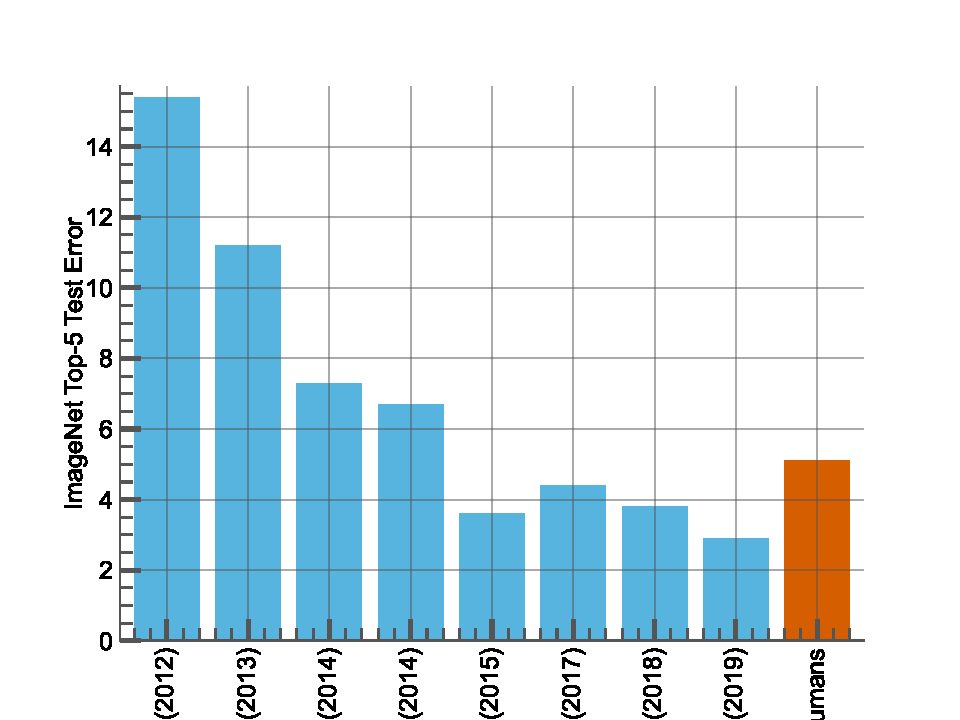
\includegraphics[width=0.8\textwidth]{chapter_intro/assets/models_vs_human.pdf}
    \caption{Models top-5 accuracy on ImageNet \cite{deng2009imagenet} compared
        to human performance.}
    \label{fig:intro:models_vs_humans}
\end{figure}

Given the nature of tasks the Netatmo cameras are designed to perform, deep
learning and \aclp{DNN} are not just a choice but a necessity. They represent
the state of the art in computer vision tasks that outperforms other algorithms
and allows for accurate and reliable object detection and recognition.\\

% \section{Challenges}

% While deep learning, particularly through the use of Convolutional Neural
% Networks (CNNs), is the technology of choice for computer vision applications,
% it comes with its set of challenges that need to be addressed, especially in the
% context of deploying these models on embedded devices. These challenges include,
% but are not limited to, model complexity, computational requirements, power
% consumption, data privacy, and real-time processing.\\

% One of the most significant challenges in deploying deep learning models,
% especially CNNs, on embedded devices, is the large model size. These models
% often have millions of parameters, making them computationally heavy and
% challenging to fit into the limited memory of embedded devices.\\

% Secondly, these complex models require substantial computational resources to
% operate. This translates into high energy consumption, a critical issue for
% battery-powered devices. Balancing the demand for high-performing models against
% the constraints of power consumption becomes a significant challenge.\\

% Data privacy presents another challenge. While it is possible to process data on
% remote servers, doing so can raise serious privacy concerns. In the context of
% Netatmo's security cameras, the data being processed can be sensitive, as it can
% involve recognising faces or detecting objects in private spaces.\\

% Another consideration is the need for real-time processing. For security
% cameras, it is crucial to detect and alert anomalies in real-time. High latency
% can lead to delayed alerts, reducing the effectiveness of the security system.\\

% Lastly, the deployment of deep learning models on embedded devices must be
% robust to environmental changes and adaptable to new situations. It is crucial
% to ensure that the performance of these models remains consistent in different
% conditions.\\

% To conclude, while deep learning and CNNs represent an exciting frontier in
% computer vision applications, several challenges need to be addressed for
% efficient and effective deployment on embedded devices. Addressing these
% challenges forms the crux of this research, with a particular focus on model
% compression techniques to reduce the size and complexity of neural networks
% without significant loss in performance.\\


\section{Contributions}

This thesis tackles the challenge of compressing \acp{DNN} through pruning, a
technique that aims to reduce the size of a neural network by removing redundant
or unnecessary parameters, subsequently detailed in \cref{chap:sota}. The
contribution detailed in this manuscript focuses on the method to identify the
parameters to prune as well as minimise the impact of their removal on the final
performance. These contributions are as follows:\\

\noindent \textbf{Budget-aware pruning with weight reparametrisation.} The two
main challenges when pruning a neural network are first, determining which
weights should be removed and then, mitigating the loss of performance
introduced by weight removal. The first challenge is often referred to as
determining the saliency of the weights. The latter is a score that reflects the
importance of the weight in the network. The second challenge is often
sidestepped and the pruned network is simply fine-tuned to recover the lost
performance. To address these challenges we propose three main contributions:

\begin{itemize}
    \item A numerically stable reparametrisation function, used in our weight
          reparametrisation and budget regularisation loss (subsequently
          detailed), that acts as a surrogate differentiable $\ell_0$ norm.

    \item A weight reparametrisation that embeds the saliency score of the
          weight in its expression and therefore value. This reparametrisation
          allows to soft-prune the weights during training thereby significantly
          mitigating the performance drop that occurs after pruning.

    \item A budget regularisation loss that allows to drive the optimisation
          procedure to respect a given budget. This budget regularisation
          benefits directly from the aforementioned reparametrisation function
          to compute the current weight budget.

    \item A comprehensive set of experiments that demonstrate the effectiveness
          of our method and its components on various datasets and
          architectures.\\
\end{itemize}

\noindent These contributions have been published in the following article:
\begin{itemize}
    \item Robin Dupont, Hichem Sahbi, and Guillaume Michel. Weight reparametrization for
          budget-aware network pruning. In \emph{2021 IEEE International Conference on Image
              Processing, ICIP 2021, Anchorage, AK, USA, September 19-22, 2021}, pages 789–793.
          IEEE, 2021.\\
\end{itemize}



\noindent \textbf{Pruning without weight training with stochastic sampling.} As
mentioned above, a major hurdle in pruning is determining which weights to
remove. This is especially challenging since weights, and consequently their
saliency, can fluctuate throughout training. This implies that pruning should
either be reversible or performed at the end of training. We propose a different
approach that does not require training the network to determine the saliency of
the weights, the latter being fixed throughout the process. Instead, we sample
subset of weights (effectively pruning the other weights) forming a subnetwork
of the original network and evaluate its performance. This allows us to search
for a topology that is both lightweight and performant inside the original
network without training the network. The main contributions of this method are
as follows: \\

\begin{itemize}
    \item A stochastic weight sampling method that is computationally efficient,
          numerically stable, differentiable and allows sampling weights while
          training their probability of being selected.
    \item An efficient learnt-based weight rescaling mechanism to compensate for
          the disruption in weight distribution statistics caused by stochastic
          sampling.
    \item A comprehensive set of experiments that demonstrate the effectiveness
          of our method and its components on various datasets and architectures, as
          well as comparison with other state-of-the-art methods in various
          configurations.
    \item A public repository containing the implementation of our method and
          the method we compare against, as well as detailed code and instructions to
          reproduce our results.\\
\end{itemize}

\noindent These contributions have been published in the following article:
\begin{itemize}
    \item Robin Dupont, Mohammed Amine Alaoui, Hichem Sahbi, and Alice
          Lebois. Extracting effective subnetworks with Gumbel-Softmax. In \textit{2022
              IEEE International Conference on Image Processing, ICIP 2022, Bordeaux,
              France, 16-19 October 2022,} pages 931–935. IEEE, 2022.\\
\end{itemize}

\section{Outline}

The rest of this thesis is organised as follows:\\

\Cref{chap:dlo} offers an introduction to deep learning, providing a detailed
overview of its foundational and core concepts. It explores early architectures,
beginning with the \emph{Perceptron} and the \ac{MLP}. The focus of the chapter
then shifts towards neural network training, giving formal definitions of the
loss function, regularisation, and optimisation process. A dedicated section
delves into \aclp{CNN}, exposing and detailing their building blocks, and the
evolution of their architectures. Then, the architectures used in the
experiments of \cref{chap:chapter1,chap:chapter2} are detailed. Additionally,
this chapter lists and describes prominent datasets, namely CIFAR-10, CIFAR-100,
and TinyImageNet, and discusses their respective train, validation, and test
sets.\\

\Cref{chap:sota} introduces deep neural network compression and presents
state-of-the-art methods divided into different families. The chapter begins
with acceleration techniques and presents a range of methods whose goal is to
speed up matrix operations or convolutions. Then, it explores the teaching
paradigm, highlighting methods that rely on a pre-trained large network to
improve the training of lightweight ones. Furthermore, the chapter addresses the
design aspects of lightweight architectures introducing building blocks for
efficient architecture design and \acl{NAS}. Afterwards, the chapter discusses
methods to compress and optimise existing architectures and in particular
pruning. Finally, the chapter presents the positioning of our methods and the
rationale behind them.\\

\Cref{chap:chapter1} presents our pruning method based on weight
reparametrisation and budget regularisation. It starts by outlining closely
related works. Then, the core methods components are examined, starting with our
weight reparametrisation and then our budget loss. Afterwards, a general
overview of the algorithm is provided. Furthermore, the chapter details
experiments assessing our method performance in various configurations as well
as experiments validating the components of our methods and the choices of
hyperparameters. A conclusion summarises the key findings and highlights of our
method for neural network pruning.\\

\Cref{chap:chapter2} delves into our stochastic pruning method without weight
training. It starts with an introduction and examination of closely related
works. Then, it details the first core component of our method, namely
\acl{ASLP}, a method for extracting effective subnetworks using the
Gumbel-Softmax technique that solves various issues that arose from previous
methods. Afterwards, it introduces our weight-rescaling technique and presents
its main benefits, as well as our pruning strategy to freeze the stochastic
topology. Subsequently, a method and algorithm overview outlines the key points
of our methods. Furthermore, the chapter exposes a comprehensive set of
experiments that compares our method against other state-of-the-art methods in
various scenarios, validates the components of our method. The chapter concludes
by summarising our findings and results.\\